\documentclass[11pt]{article}
\usepackage[english]{babel}
\usepackage[utf8]{inputenc}
\usepackage{fancyhdr}
\usepackage{graphicx}

\def\Name{Ran Liao}
\def\Topic{Classical Analysis}

\title{\textbf{\Topic}}
\author{\Name}
\markboth{Notes on \Topic\ }{Notes on \Topic\ }
\date{\today}
 
\pagestyle{fancy}
\fancyhf{}
\rhead{\date{\today} }
\lhead{Notes on \Topic\ }
\rfoot{\thepage}

\textheight=9in
%\textwidth=6.5in
\topmargin=-.75in
%\oddsidemargin=0in
%\evensidemargin=0in
 
\begin{document}
\maketitle
\noindent\makebox[\linewidth]{\rule[8pt]{5in}{0.5pt}}

\section*{Data Flow Diagram}

The data flow diagram shows the logical data flow.

\begin{figure}[h]
	\begin{minipage}[t]{0.4\linewidth}
	\centering 
	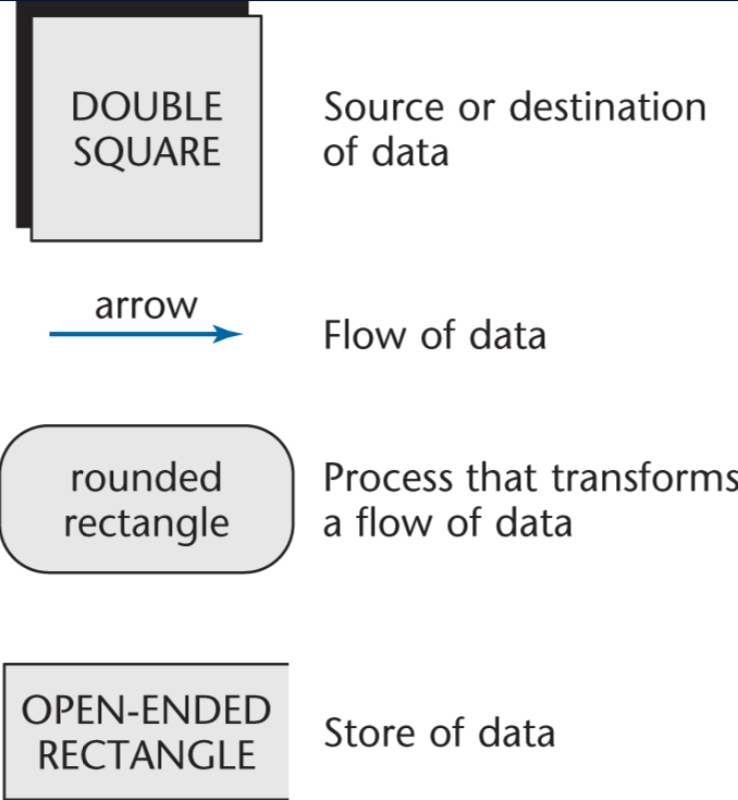
\includegraphics[width=1.2\textwidth]{images/DataFlowDiagramSymbol.png}
	\caption{Symbol}
	\label{fig:DataFlowDiagramSymbol}
	\end{minipage} 
	\hfill
	\begin{minipage}[t]{0.4\linewidth}
	\centering
	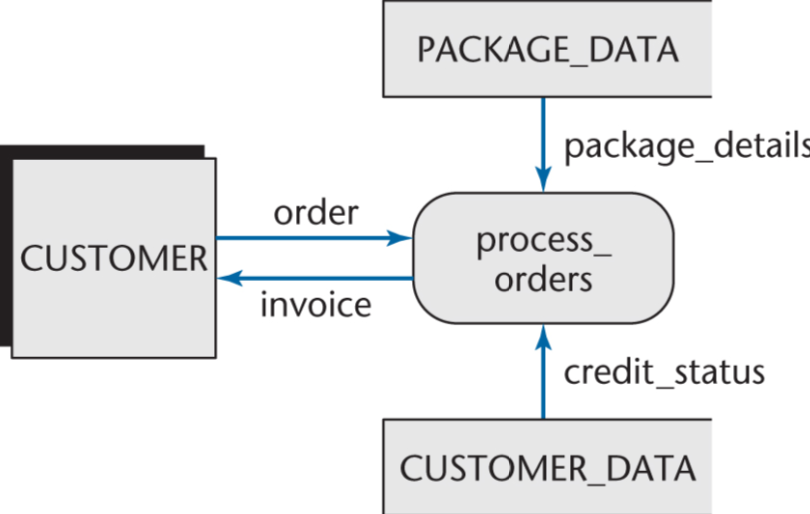
\includegraphics[width=1.2\textwidth]{images/DataFlowDiagram.png}
	\caption{Data Flow Diagram} 
	\label{fig:DataFlowDiagram}
	\end{minipage}
\end{figure}

\newpage
\section*{Data Flow Analysis}

\begin{enumerate}

	\item Determine ``Point of highest abstraction of input" and ``Point of highest abstract of output".
	
	\begin{figure}[h]
		\centering
		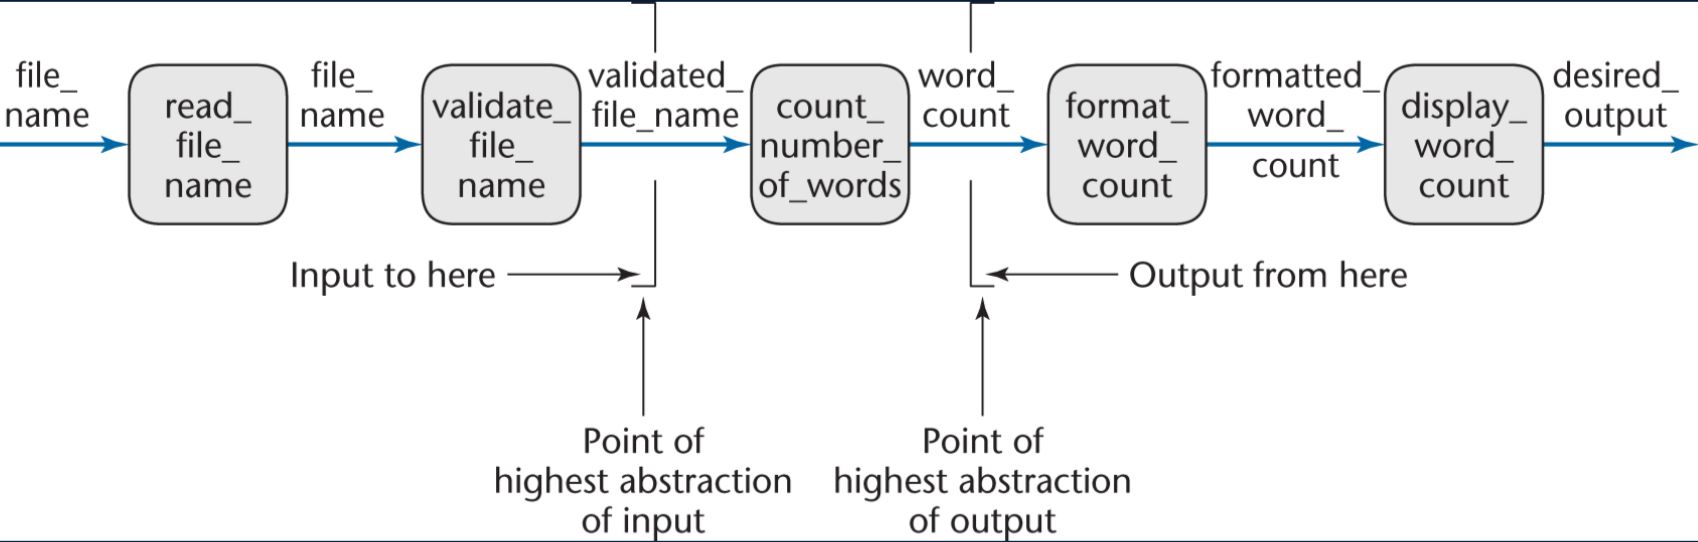
\includegraphics[width=0.8\linewidth]{images/DataFlowAnalysis.png}
		\caption{Data Flow Analysis}
		\label{fig:DataFlowAnalysis}
	\end{figure}
	
	\item Decompose the product into three modules.
	
	\begin{figure}[h]
		\centering
		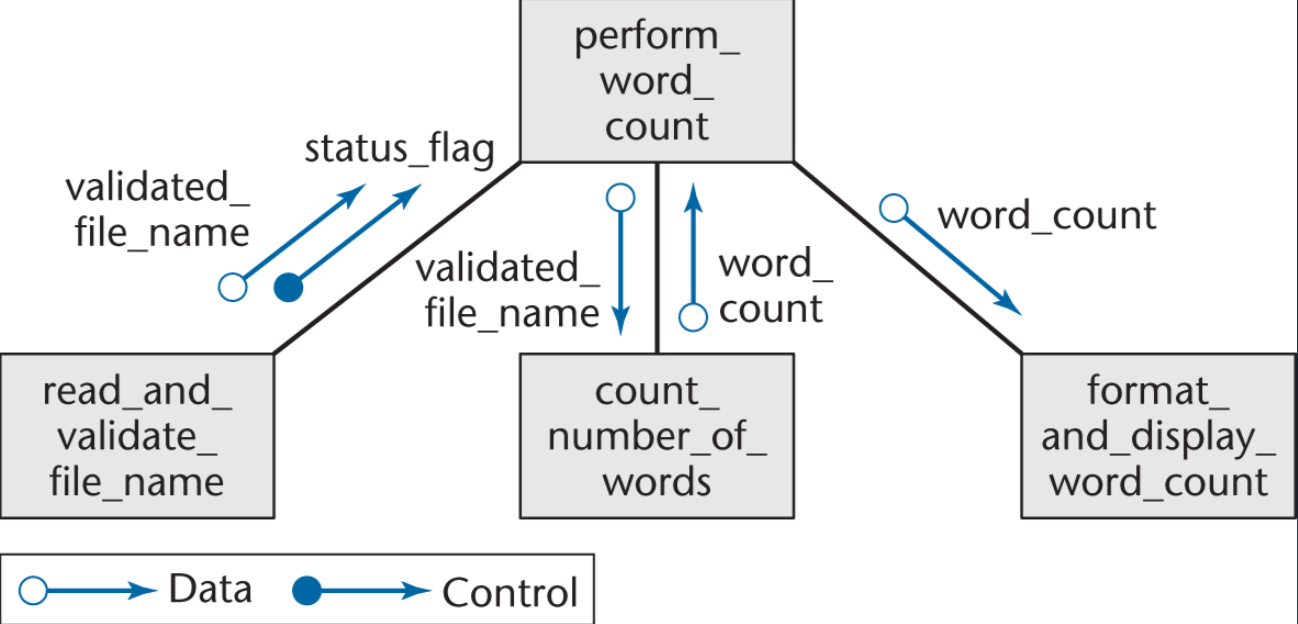
\includegraphics[width=0.8\linewidth]{images/FirstRefinements.png}
		\caption{First Refinement}
		\label{fig:FirstRefinements}
	\end{figure}
	
	\item Repeat stepwise until each module has high cohesiom

	\begin{figure}[h]
		\centering
		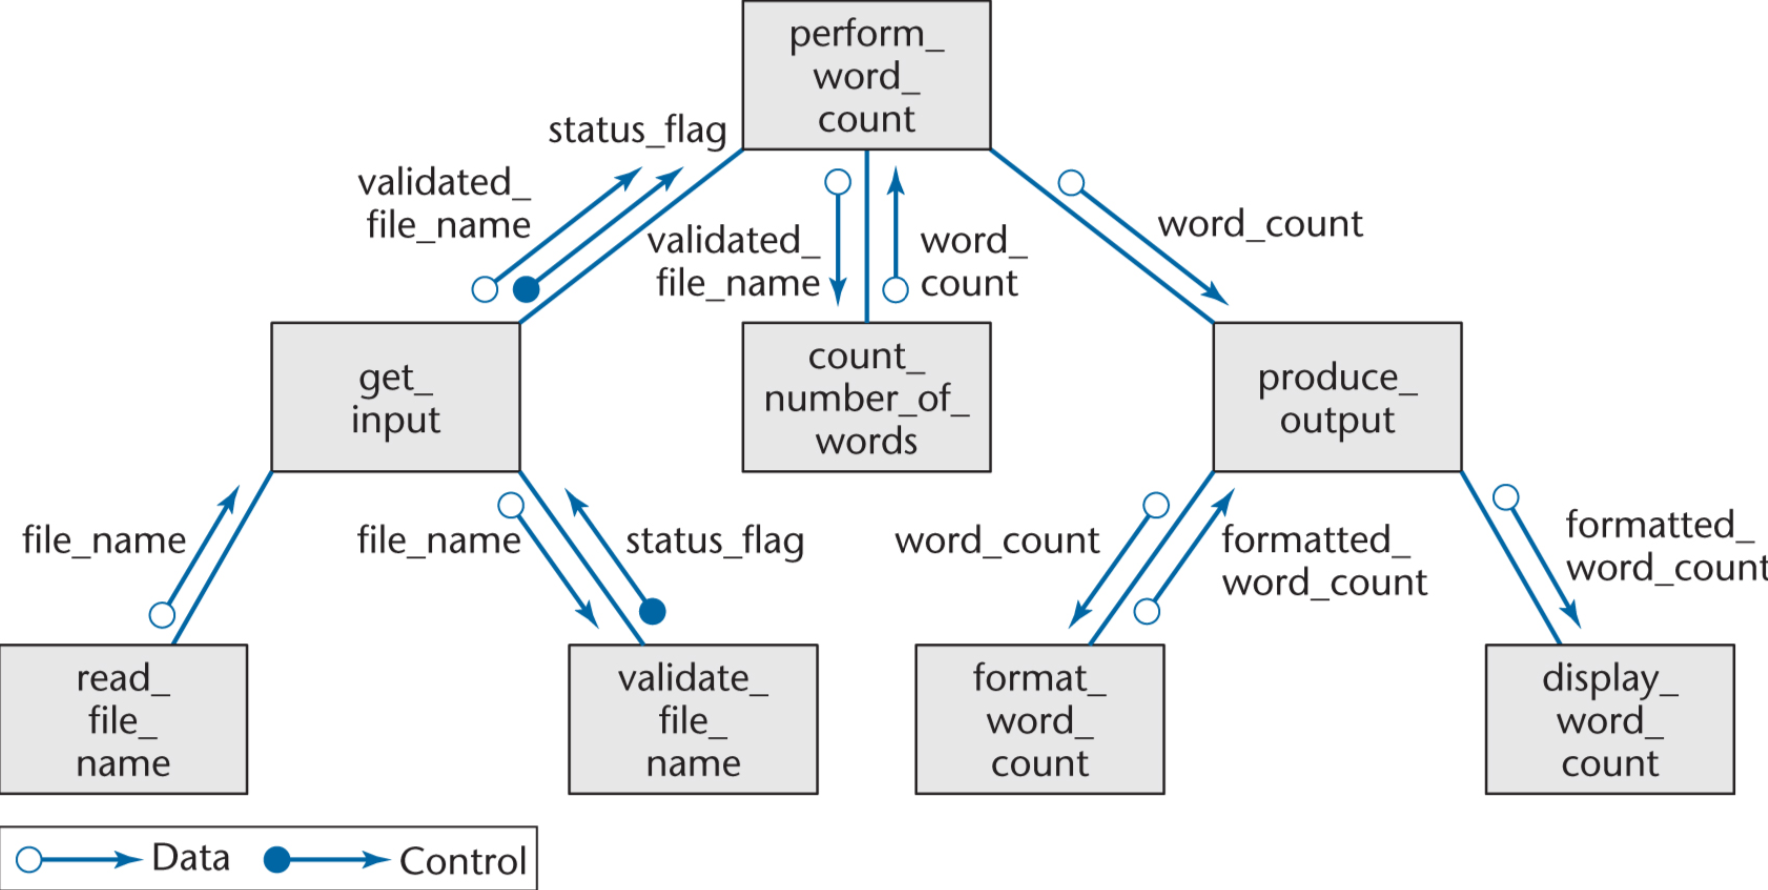
\includegraphics[width=0.8\linewidth]{images/SecondRefinements.png}
		\caption{Second Refinement}
		\label{fig:SecondRefinements}
	\end{figure}

\end{enumerate}












\end{document}